\formdesc{Mode Commun et Différentiel  : }

\begin{enumerate}
    \item Commun : par rapport à la GND
    \item Différentiel : entre deux potentiels 
\end{enumerate}

\formtitle{Schéma bloc}


\vspace{-5mm}

\begin{center}
    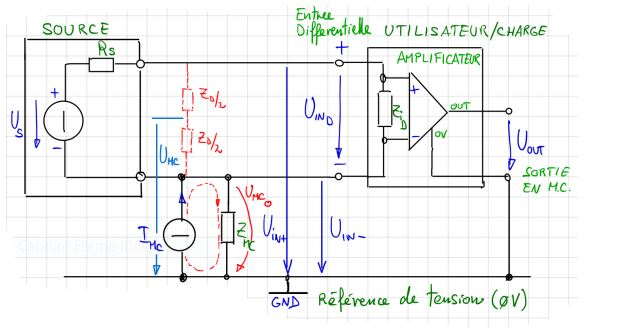
\includegraphics[width = 0.54\textwidth]{img/Schéma.JPG}
\end{center}

Tension mode commun : 
{\hfill$ U_{MC}  = \cfrac{(U_{in+})+(U_{in-})}{2}$ \hfill}

{\hfill$ U_{MC_0}  = I_{MC} \cdot Z_{MC}$ \hfill}

Tension différentielle : 

{\hfill$ U_{D}  = (U_{in+}).(U_{in-})$ \hfill}

\formtitle{Commun Mode Rejection Ratio : CMRR }

Cette grandeur donne l’atténuation d’un signal en entrée en MC sur la sortie :

{\hfill$ CMRR = 20log_{10}\cfrac{U_{in,MC}(f)}{U_{out}(f)}$ \hfill}

\hformbar

\formdesc{Sample \& Hold}

$\Delta t_{max} = \cfrac{Dyn}{\hat{U} 2^{n_bit} \pi f_{in}}$\\

$\Delta u =  \hat{U}2 \pi f_{in} \Delta t $  \\

$SNR_{jig} = -20log(2 \pi f_{in} \Delta t)$

\formdesc{Sigma-Delta }


\formtitle{Ordre 1 }

$SNRQ = 10log(\cfrac{\sigma_x^2}{Vref^2})+ 5.6 + 30log(NOSR)$


\formtitle{Ordre 2 }

$SNRQ = 10log(\cfrac{\sigma_x^2}{Vref^2})- 2.1  + 50log(NOSR)$

\hformbar

\formdesc{Cascaded Integrator Comb Filter }

\vspace{-5mm}
\begin{center}
    \hspace{-2cm}    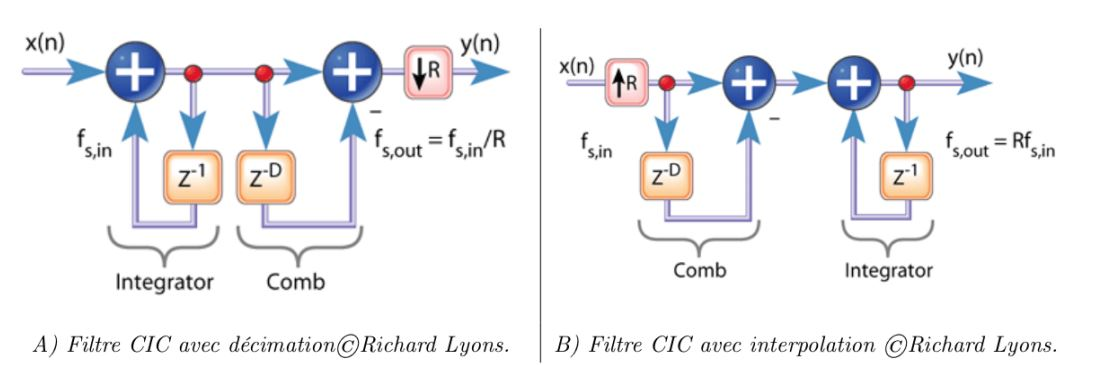
\includegraphics[width = 0.6\textwidth]{img/CIC_Z.JPG}
\end{center}

\vspace{-10mm}

\begin{center}
    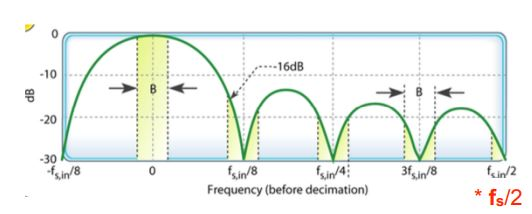
\includegraphics[width = 0.5\textwidth]{img/sinus_card.JPG}
\end{center}

\vspace{-5mm}

*dans ces figures $Fs,in$ est la fréquence du bitstream $fs = NOSR \cdot FS$ en entrée du filtre CIC.

Exemple pour D = 8 donc creux à tous les $f =\cfrac{k}{8}$


\formtitle{Avec Sigma-Delta}

\vspace{-3mm}

\begin{center}
    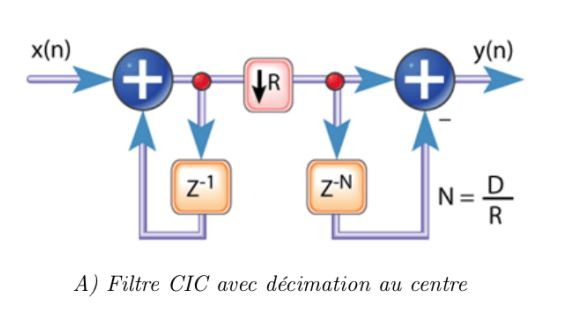
\includegraphics[width = 0.3\textwidth]{img/CIC_centre.JPG}
\end{center}


\vspace{-5mm}

\begin{center}
    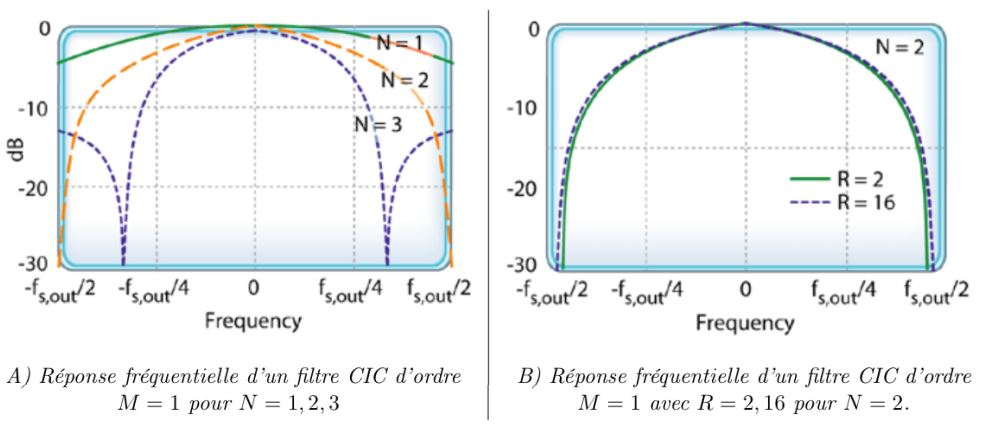
\includegraphics[angle=90,width = 0.3\textwidth]{img/cic_avecDelta.JPG}
\end{center}

La plupart du temps on a R = D donc N = 1

M  = ordre filtre CIC
\begin{center}
    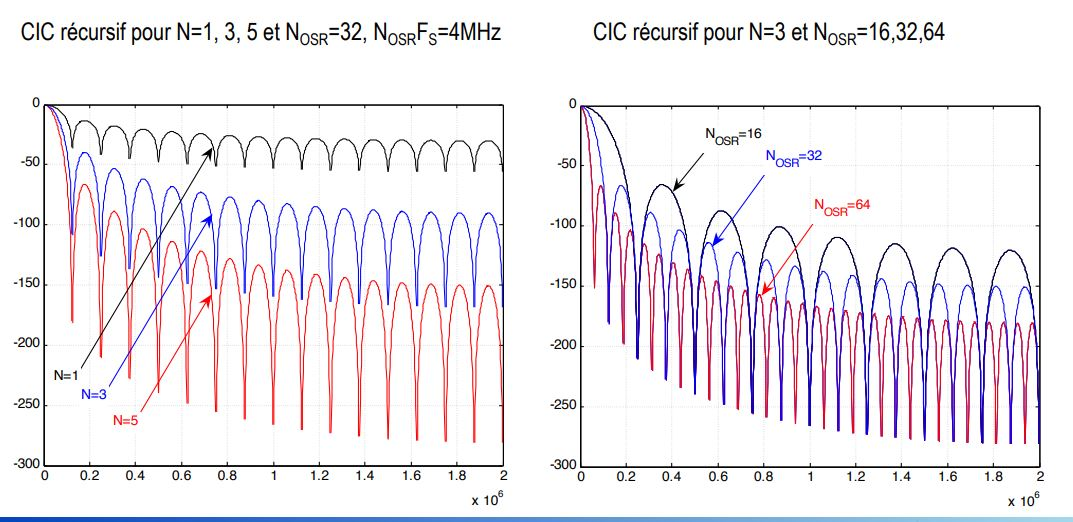
\includegraphics[angle=90,width = 0.3\textwidth]{img/Sook.JPG}
\end{center}